\documentclass[12pt,a4paper]{article}

% ─────────────────────────────────────────────────────────────
%  Processamento Digital de Imagens Ambientais com Python
%  Avaliação A3 — Computação Gráfica
%  Compilar no Overleaf com pdfLaTeX
% ─────────────────────────────────────────────────────────────

\usepackage[utf8]{inputenc}
\usepackage[T1]{fontenc}
\usepackage[brazil]{babel}
\usepackage[a4paper,margin=2.5cm]{geometry}
\usepackage{graphicx}
\usepackage{booktabs}
\usepackage{float}
\usepackage{amsmath}
\usepackage{siunitx}
\usepackage{caption}
\usepackage{subcaption}
\usepackage{xcolor}
\usepackage{listings}
\usepackage[hidelinks]{hyperref}
\usepackage{setspace}

\graphicspath{{figuras/}}
\onehalfspacing

% Estilo para trechos de código
\definecolor{codegray}{gray}{0.95}
\lstset{
  basicstyle=\ttfamily\small,
  backgroundcolor=\color{codegray},
  frame=single,
  breaklines=true,
  language=Python,
  showstringspaces=false,
}

\title{\textbf{Processamento Digital de Imagens Ambientais com Python}\\
\large Segmentação de Vegetação por Índices Espectrais VARI e ExG}

\author{
  Gilberto de Paiva Melo \\
  \small Matrícula: \rule{3cm}{0.4pt} \quad Turma: \rule{2cm}{0.4pt} \\
  \small Curso de Ciência da Computação --- Computação Gráfica \\
  \small Avaliação A3 --- Semestre 2025.1
}
\date{\today}

\begin{document}

\maketitle

\begin{abstract}
\noindent
Este trabalho apresenta um \emph{pipeline} completo de processamento digital de imagens
para análise de cobertura vegetal a partir de fotografias RGB, implementado em Python com
OpenCV, NumPy, Matplotlib e scikit-image. O sistema realiza aquisição, pré-processamento,
análise de histograma, filtragem comparativa (Gaussiano, Mediana e Bilateral), detecção de
bordas (Canny), e segmentação de vegetação por índices espectrais de crominância (VARI e ExG).
Demonstra-se empiricamente que índices de crominância superam a limiarização de Otsu por
luminância na distinção de vegetação, e propõe-se uma segmentação aprimorada combinando o
índice ExGR com uma trava de cor em HSV, capaz de eliminar falsos positivos em solo, céu e
superfícies acinzentadas. Os experimentos cobrem seis imagens de origem diversa (câmera de
celular e drone), evidenciando que a escolha do tipo de imagem é parte integrante do algoritmo.
\\[1ex]
\textbf{Palavras-chave:} visão computacional; índices de vegetação; VARI; ExG; segmentação; OpenCV.
\end{abstract}

\tableofcontents
\newpage

% ════════════════════════════════════════════════════════════
\section{Introdução e Contextualização}
% ════════════════════════════════════════════════════════════

A Computação Gráfica é a área da Ciência da Computação responsável pela geração, manipulação
e análise de imagens por meio de algoritmos. No contexto atual, a visão computacional e o
processamento digital de imagens permeiam aplicações que vão de diagnósticos médicos ao
monitoramento de ecossistemas.

Este projeto integra a \textbf{captura real de imagens} --- realizada pelo próprio aluno com
câmera de smartphone --- ao posterior tratamento digital em Python. O fio condutor é ambiental:
quantificar a cobertura vegetal de uma cena diretamente a partir de uma fotografia comum,
sem sensores especializados. Tal capacidade tem relevância em agricultura de precisão,
monitoramento de desmatamento e análise de áreas verdes urbanas, onde imagens de satélite são
caras e pouco frequentes, enquanto um celular captura milhões de pixels instantaneamente.

O olho humano distingue o verde com facilidade, mas o computador enxerga apenas números. O
objetivo central é transformar esses números em uma resposta objetiva: \emph{quais pixels
correspondem a vegetação e qual o percentual de cobertura.}

% ════════════════════════════════════════════════════════════
\section{Objetivos}
% ════════════════════════════════════════════════════════════

\subsection{Objetivo Geral}
Desenvolver um sistema de processamento digital de imagens em Python capaz de analisar imagens
capturadas pelo aluno, aplicando técnicas de Computação Gráfica para extrair informação
quantitativa de vegetação e realizar tratamentos visuais com fins analíticos e ambientais.

\subsection{Objetivos Específicos}
\begin{itemize}
  \item Capturar imagens reais com participação ativa do aluno, documentando equipamentos;
  \item Implementar pré-processamento: leitura, conversão de espaço de cores, redimensionamento
        e normalização;
  \item Aplicar ao menos quatro técnicas distintas: filtros de suavização, detecção de bordas,
        transformações morfológicas e análise de histograma;
  \item Realizar segmentação de regiões de interesse por limiarização (Otsu) e por índices
        espectrais;
  \item Apresentar resultados comparativos (original $\times$ processado) com análise crítica;
  \item Documentar todo o processo em relatório técnico e código comentado.
\end{itemize}

% ════════════════════════════════════════════════════════════
\section{Fundamentação Teórica}
% ════════════════════════════════════════════════════════════

\subsection{Imagem digital e o modelo RGB}
Uma imagem digital é uma representação matricial de uma cena, composta por \emph{pixels}. Em
imagens coloridas no modelo RGB, cada pixel é descrito por três canais --- Vermelho (R),
Verde (G) e Azul (B) --- com valores inteiros de 0 a 255 (8 bits por canal), totalizando até
16,7 milhões de cores. No NumPy, a imagem é um arranjo de forma $(altura, largura, 3)$.

\subsection{Espaços de cor}
\begin{itemize}
  \item \textbf{RGB:} modelo aditivo padrão de câmeras e monitores. Mistura cor e brilho nos
        três canais, dificultando isolar matizes específicos.
  \item \textbf{Escala de cinza:} intensidade luminosa única por pixel, obtida por média
        ponderada ($0{,}299R + 0{,}587G + 0{,}114B$).
  \item \textbf{HSV (Matiz, Saturação, Valor):} separa a cor em três eixos perceptuais. Um
        pixel acinzentado tem saturação próxima de zero independentemente do brilho, o que
        permite rejeitar superfícies neutras com uma regra simples sobre o canal $S$.
\end{itemize}

\subsection{Índices de vegetação}
Folhas saudáveis refletem mais verde e absorvem mais vermelho (clorofila). Índices de vegetação
exploram essa assinatura espectral.

\paragraph{VARI --- Visible Atmospherically Resistant Index} \cite{gitelson2002}
\begin{equation}
\text{VARI} = \frac{G - R}{G + R - B + \varepsilon}
\end{equation}
Varia de $-1$ a $+1$; valores positivos indicam vegetação. O termo $\varepsilon = 10^{-6}$
evita divisão por zero. É resistente a variações de iluminação atmosférica.

\paragraph{ExG --- Excess Green Index} \cite{woebbecke1995}
\begin{equation}
\text{ExG} = 2G - R - B
\end{equation}
Simples e de baixo custo, com limiar natural em zero para segmentação.

\paragraph{ExGR --- Excess Green minus Excess Red} \cite{meyer2008}
\begin{equation}
\text{ExR} = 1{,}4R - G \qquad \text{ExGR} = \text{ExG} - \text{ExR} = 3G - 2{,}4R - B
\end{equation}
Subtrai o excesso de vermelho, alto em solo e palha, separando melhor vegetação de fundo.

\subsection{Filtros de suavização}
\begin{itemize}
  \item \textbf{Gaussiano:} convolução com \emph{kernel} gaussiano; reduz ruído de alta
        frequência borrando indiscriminadamente.
  \item \textbf{Mediana:} substitui cada pixel pela mediana da vizinhança; eficaz contra ruído
        impulsivo, preserva bordas.
  \item \textbf{Bilateral:} média ponderada que respeita diferenças de cor; suaviza preservando
        bordas.
\end{itemize}

\subsection{Detecção de bordas --- Canny}
O operador de Canny suaviza a imagem, calcula o gradiente, aplica supressão de não-máximos e
usa histerese com dois limiares para conectar bordas fortes e fracas, evitando contornos
quebrados.

\subsection{Limiarização de Otsu}
Otsu testa todos os limiares possíveis e escolhe o que \textbf{maximiza a variância entre as
duas classes} de intensidade. Requer histograma bimodal para funcionar bem.

\subsection{Morfologia matemática}
Operações sobre máscaras binárias com um elemento estruturante. A \emph{abertura}
(erosão seguida de dilatação) remove ruído; o \emph{fechamento} (dilatação seguida de erosão)
preenche buracos.

\subsection{Métricas de fidelidade --- PSNR e SNR}
\begin{equation}
\text{PSNR} = 10\log_{10}\!\left(\frac{\text{MAX}^2}{\text{MSE}}\right)
\qquad
\text{SNR} = 10\log_{10}\!\left(\frac{P_{\text{sinal}}}{P_{\text{ruído}}}\right)
\end{equation}
Ambas medem, em decibéis, o quanto a imagem filtrada se afasta da original: valores maiores
indicam maior fidelidade.

% ════════════════════════════════════════════════════════════
\section{Metodologia}
% ════════════════════════════════════════════════════════════

\subsection{Ferramentas}
O projeto foi desenvolvido em \textbf{Python 3.11} com as bibliotecas OpenCV 4.13,
NumPy 2.4, Matplotlib 3.10, Pillow 12.2 e scikit-image 0.26, em ambiente Jupyter Lab.

\subsection{Aquisição das imagens}
Foram capturadas três imagens com câmera de smartphone (uma paisagem vegetada e duas cenas
de teste) e selecionadas três imagens aéreas de drone para avaliar o comportamento do
\emph{pipeline} sob aquisição em ângulo \emph{nadir} (visada vertical).

\subsection{Pipeline de processamento}
\begin{enumerate}
  \item \textbf{Aquisição:} leitura com \texttt{cv2.imread()} e conversão BGR~$\rightarrow$~RGB;
  \item \textbf{Pré-processamento:} inspeção de metadados, redimensionamento com
        \texttt{cv2.resize}, conversão para escala de cinza e normalização para $[0,1]$;
  \item \textbf{Análise inicial:} histograma dos canais R, G e B;
  \item \textbf{Índices:} cálculo de VARI (com máscara de luminância) e ExG;
  \item \textbf{Filtragem:} Gaussiano ($\sigma = 1{,}5$), Mediana ($5\times5$) e Bilateral
        ($d = 9$), avaliados por PSNR e SNR;
  \item \textbf{Detecção de bordas:} Canny com limiares 50 e 130;
  \item \textbf{Segmentação:} Otsu (grayscale) \emph{vs.} ExG, com refino morfológico;
  \item \textbf{Segmentação aprimorada:} ExGR + trava HSV + preenchimento de buracos;
  \item \textbf{Visualização:} \emph{grid} comparativo de todos os estágios.
\end{enumerate}

% ════════════════════════════════════════════════════════════
\section{Resultados e Discussão}
% ════════════════════════════════════════════════════════════

\subsection{Aquisição e metadados}
A imagem principal (\texttt{paisagem-verde.jpeg}) apresentou os seguintes metadados:

\begin{table}[H]
\centering
\caption{Metadados da imagem principal.}
\begin{tabular}{ll}
\toprule
\textbf{Atributo} & \textbf{Valor} \\
\midrule
Resolução        & $2268 \times 4032$ pixels \\
Número de canais & 3 (R, G, B) \\
Tipo (dtype)     & \texttt{uint8} (0--255) \\
Tamanho em disco & 1588,2 KB \\
Pixel [100, 200] & [20, 34, 19] (verde dominante) \\
\bottomrule
\end{tabular}
\end{table}

\noindent
O redimensionamento para 1024 px de largura (mantendo a proporção) resultou em
$1024 \times 1820$ pixels, uma redução de \textbf{79,6\%} no volume de dados --- útil para
prototipagem rápida.

\subsection{Análise de histograma}
A Figura~\ref{fig:histogramas} apresenta a distribuição de intensidades dos canais R, G, B e do
índice ExG. Os três canais ocupam toda a faixa $[0,1]$; o ExG concentra-se em valores positivos
(média 0,084 na escala normalizada), confirmando dominância de verde na cena.

\begin{figure}[H]
\centering
\begin{subfigure}{0.49\textwidth}
  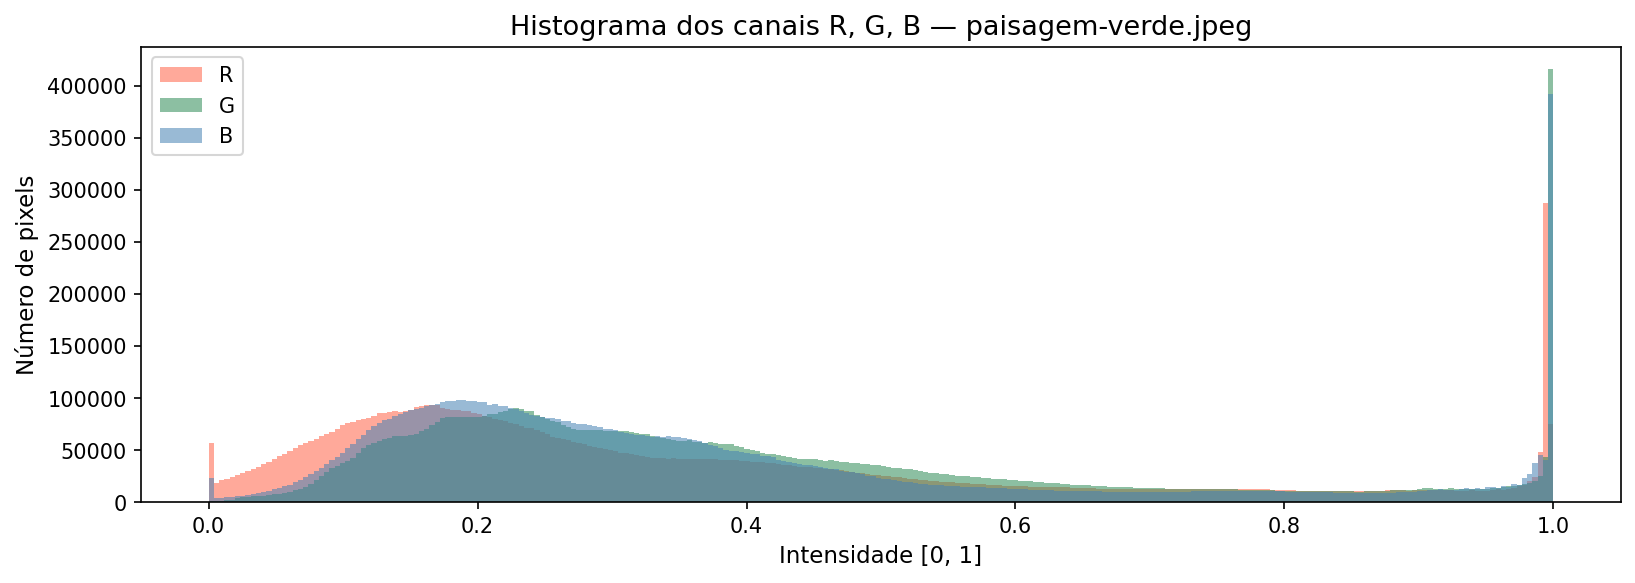
\includegraphics[width=\linewidth]{histograma_rgb.png}
  \caption{Canais R, G, B}
\end{subfigure}
\hfill
\begin{subfigure}{0.49\textwidth}
  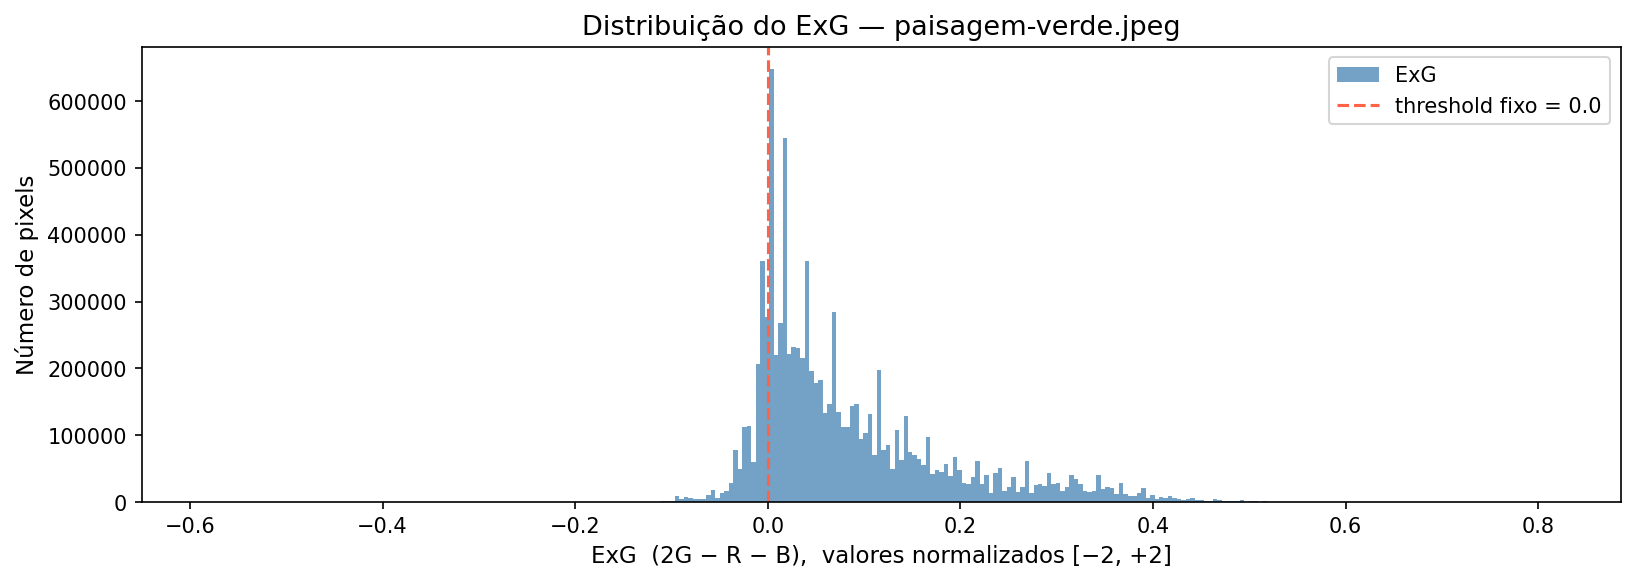
\includegraphics[width=\linewidth]{histograma_exg.png}
  \caption{Índice ExG}
\end{subfigure}
\caption{Histogramas dos canais de cor e do índice de vegetação ExG.}
\label{fig:histogramas}
\end{figure}

\subsection{Índices de vegetação}
O cálculo do VARI revelou um problema numérico relevante: em pixels de sombra, o denominador
$G + R - B$ aproxima-se de zero, gerando \emph{outliers} extremos (valores brutos de
$-11{.}764$ a $235{.}294$ antes do recorte). A solução adotada foi uma \textbf{máscara de
luminância}, que zera o índice onde $(R+G+B)/3 < 0{,}1$: foram excluídos
\textbf{521.887 pixels (5,71\%)} de sombra, alterando a média do VARI de apenas 0,2483 para
0,2453 --- confirmando que tais pixels eram ruído numérico, não sinal. A
Figura~\ref{fig:indices} mostra os mapas de VARI e ExG.

\begin{figure}[H]
\centering
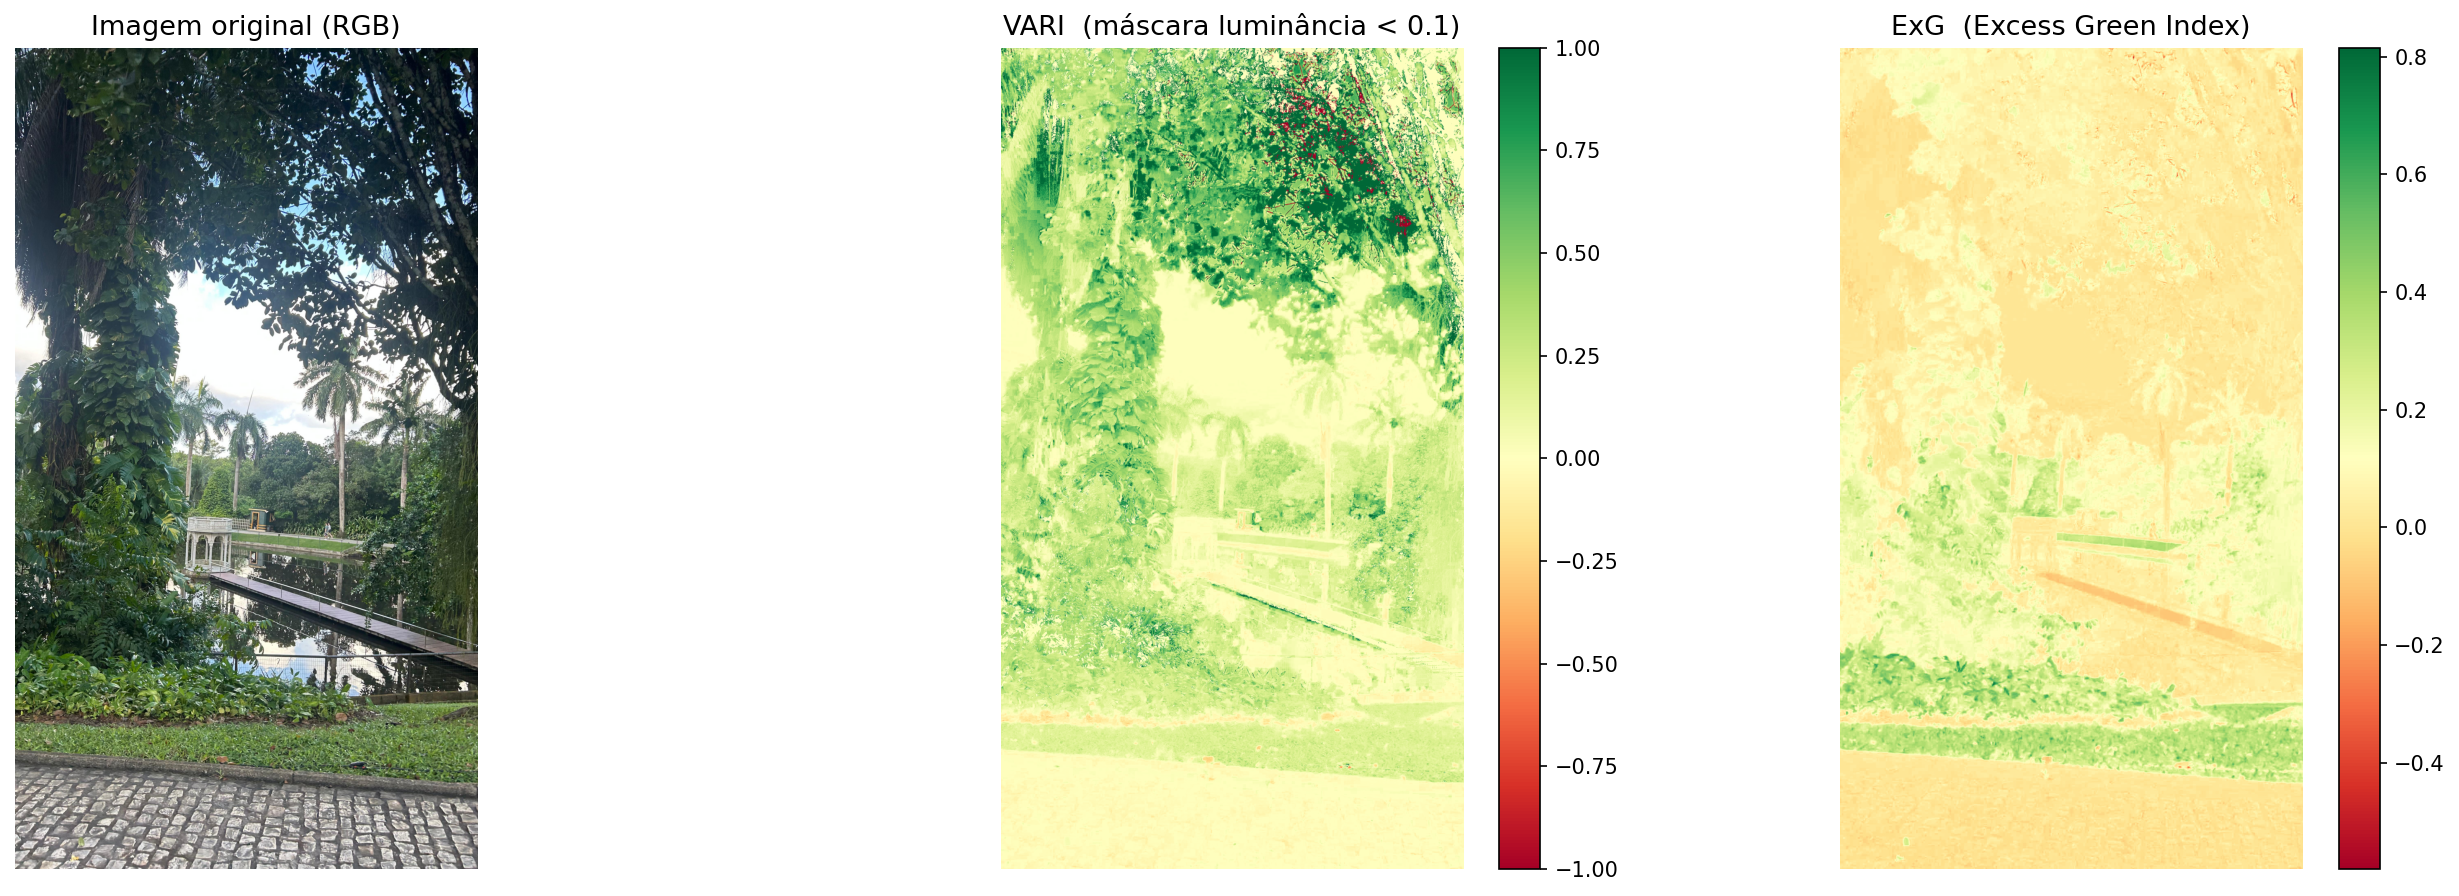
\includegraphics[width=\textwidth]{comparativo_indices.png}
\caption{Imagem original, mapa VARI (com máscara de luminância) e mapa ExG.
Escala \texttt{RdYlGn}: vermelho indica ausência e verde indica presença de vegetação.}
\label{fig:indices}
\end{figure}

\subsection{Filtragem comparativa}
A Tabela~\ref{tab:filtros} resume o desempenho dos três filtros, e a
Figura~\ref{fig:filtros} mostra o resultado visual.

\begin{table}[H]
\centering
\caption{Comparação de filtros de suavização (imagem principal).}
\label{tab:filtros}
\begin{tabular}{lccc}
\toprule
\textbf{Filtro} & \textbf{PSNR (dB)} & \textbf{SNR (dB)} & \textbf{Tempo (ms)} \\
\midrule
Gaussiano $\sigma=1{,}5$ & 25,39 & 18,66 & 50,3 \\
Mediana $5\times5$       & 26,12 & 19,39 & 63,8 \\
Bilateral $d=9$          & \textbf{32,01} & \textbf{25,27} & 109,9 \\
\bottomrule
\end{tabular}
\end{table}

\noindent
O filtro \textbf{bilateral} obteve o maior PSNR e SNR: por preservar bordas, afasta-se menos da
imagem original, sendo o mais fiel numericamente apesar de visualmente suave. O Gaussiano,
que borra indiscriminadamente, foi o menos fiel.

\begin{figure}[H]
\centering
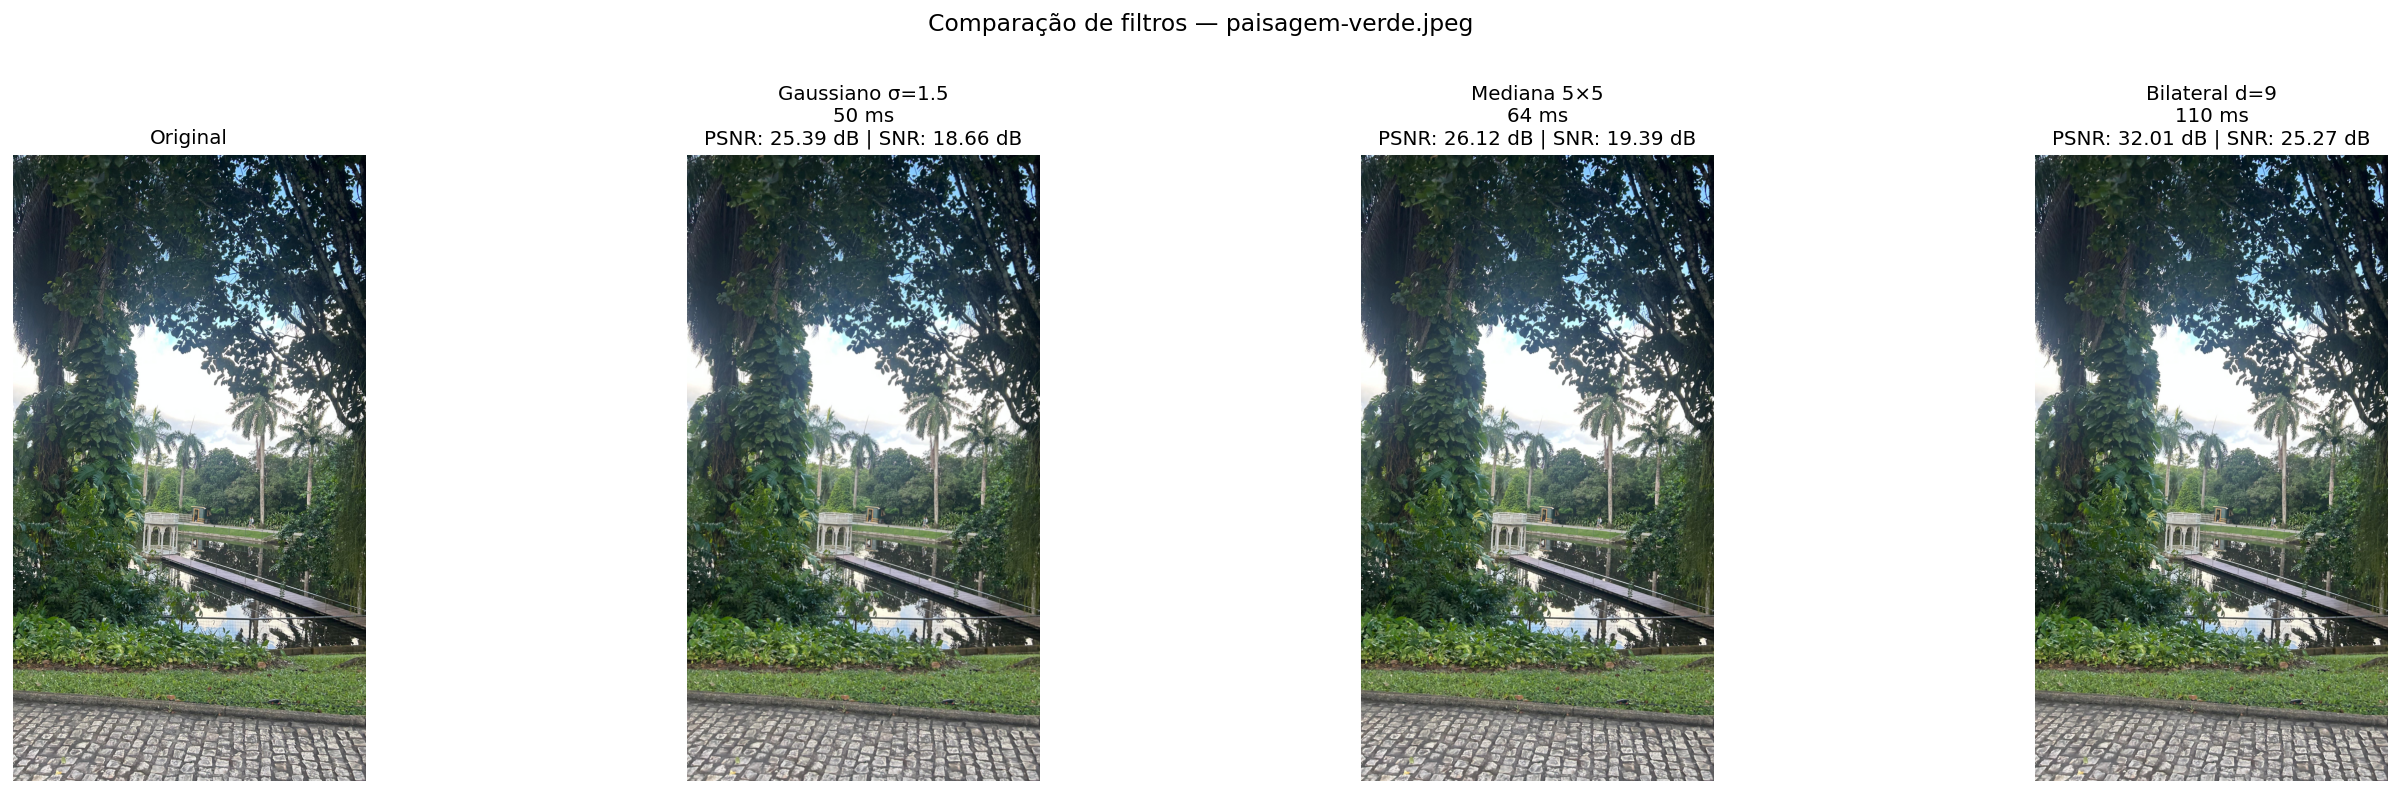
\includegraphics[width=\textwidth]{comparacao_filtros.png}
\caption{Comparação visual entre original e os filtros Gaussiano, Mediana e Bilateral.}
\label{fig:filtros}
\end{figure}

\subsection{Segmentação: Otsu \emph{vs.} ExG}
A Tabela~\ref{tab:segmentacao} e a Figura~\ref{fig:segmentacao} contrastam os dois métodos.

\begin{table}[H]
\centering
\caption{Otsu (luminância) \emph{vs.} ExG (crominância).}
\label{tab:segmentacao}
\begin{tabular}{lccc}
\toprule
\textbf{Método} & \textbf{Threshold} & \textbf{Cobertura} & \textbf{Regiões} \\
\midrule
Otsu (grayscale) & 0,5294 & 13,08\% & 259 \\
ExG fixo ($>0$)  & 0,0000 & 82,24\% & 150 \\
\bottomrule
\end{tabular}
\end{table}

\noindent
Otsu segmenta por \textbf{brilho}: o limiar 0,53 separa pixels claros de escuros, detectando
apenas 13\% e fragmentando a cena em 259 regiões. O ExG segmenta por \textbf{assinatura
espectral}, detectando 82\% em apenas 150 regiões coerentes. Conclui-se que, para imagens RGB
de campo, a limiarização por índice espectral é metodologicamente superior à de Otsu por
luminância, que descarta a informação de crominância que define a vegetação.

\begin{figure}[H]
\centering
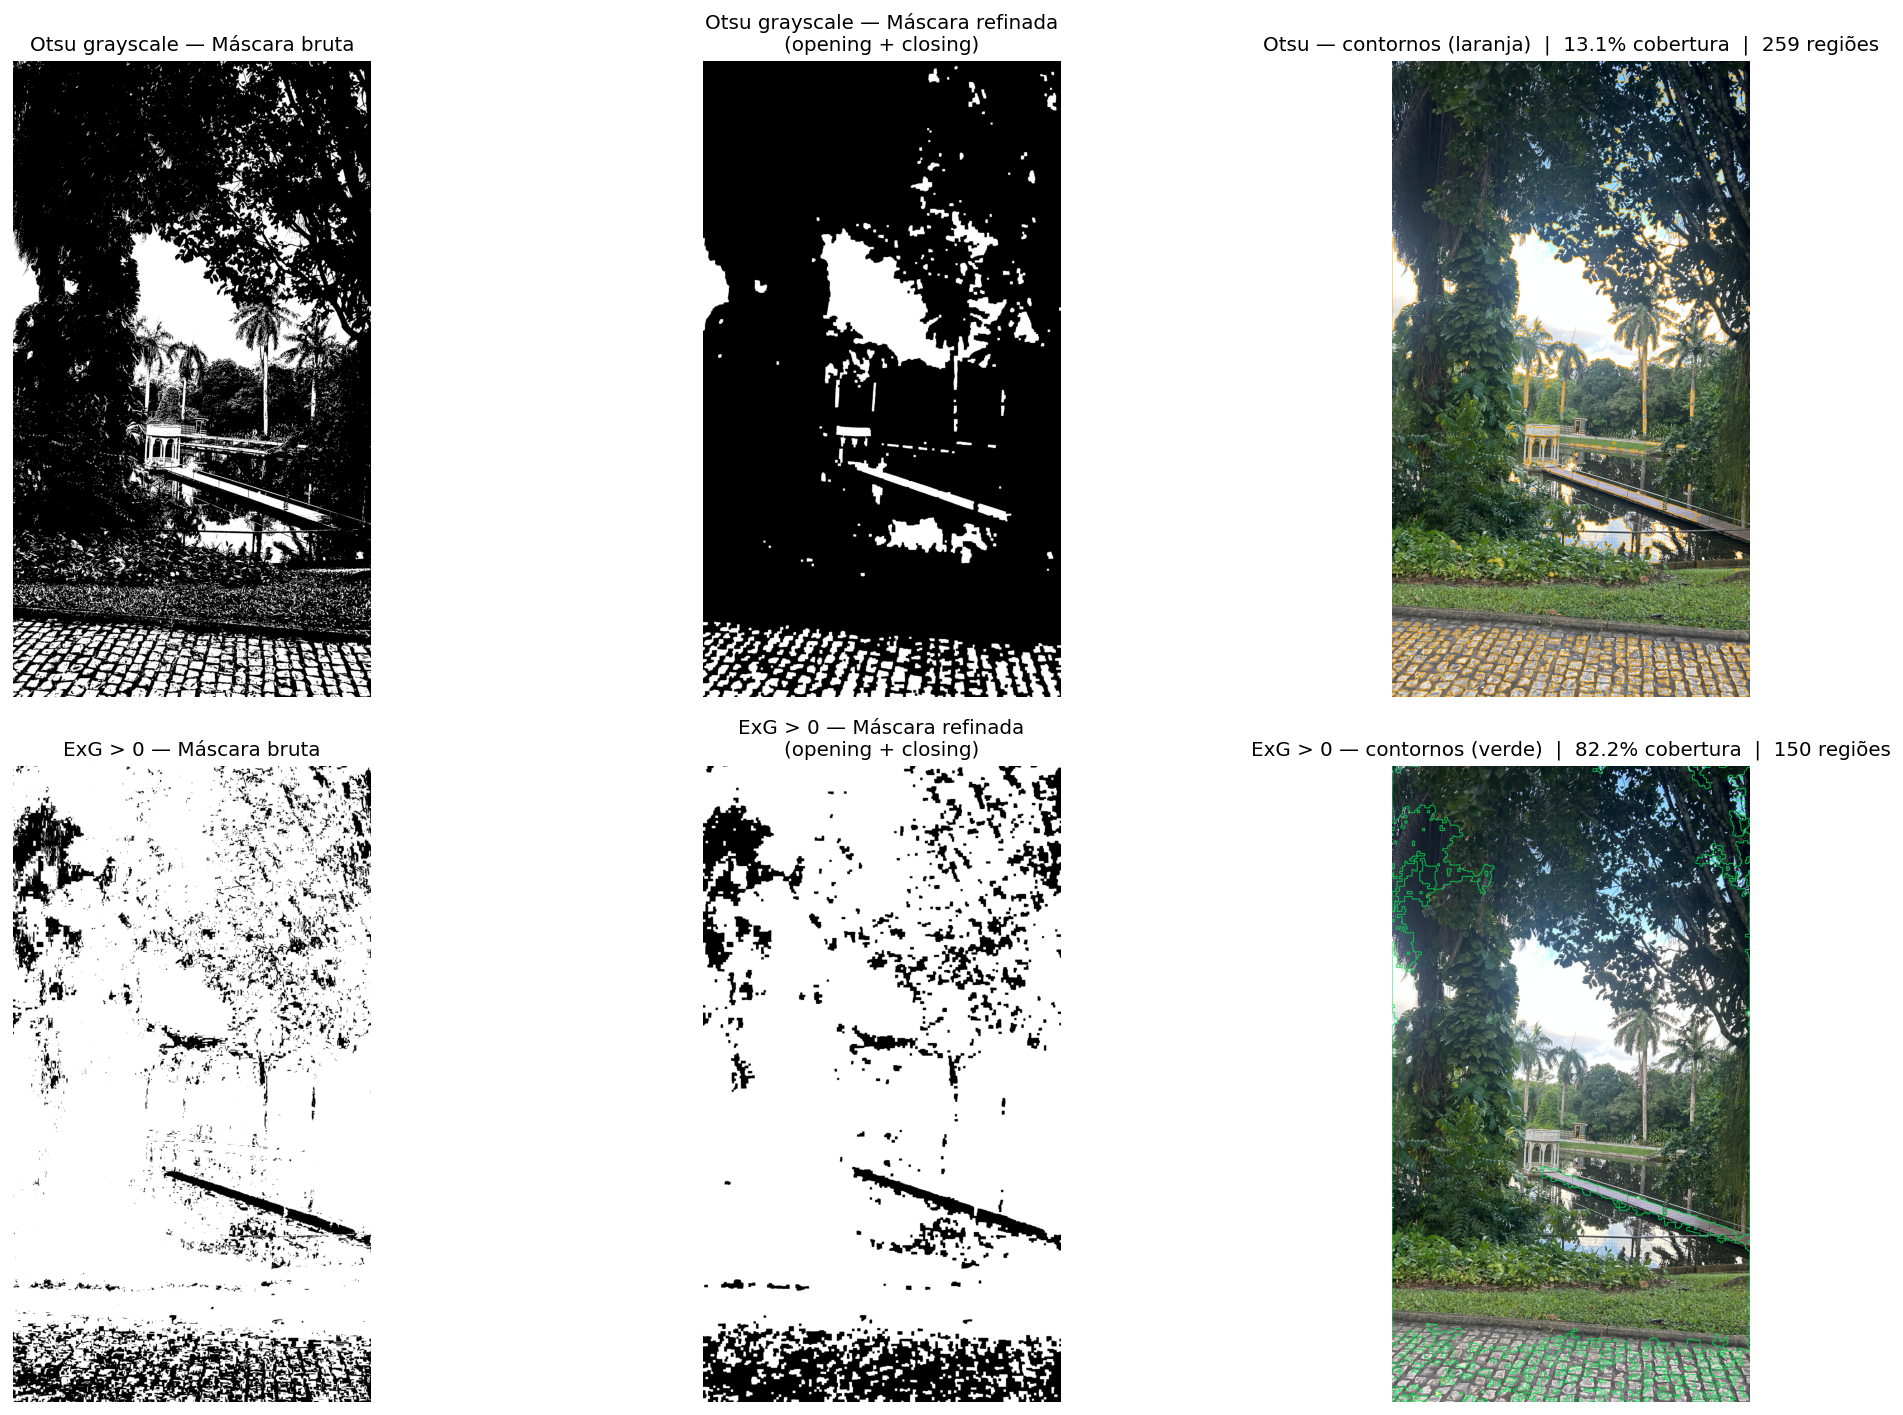
\includegraphics[width=\textwidth]{comparacao_segmentacao.png}
\caption{Máscaras de segmentação por Otsu (grayscale) e por ExG, após refino morfológico
(\texttt{MORPH\_OPEN} + \texttt{MORPH\_CLOSE}, kernel elíptico $7\times7$).}
\label{fig:segmentacao}
\end{figure}

\subsection{Segmentação aprimorada}
A segmentação ingênua ($\text{ExG} > 0$) produz \textbf{falsos positivos} em céu, solo claro e
superfícies acinzentadas. A versão aprimorada combina o índice ExGR com uma \textbf{trava de
cor em HSV} ($H \in [30,95]$, $S \geq 40$, $V \geq 30$), preenchimento de buracos e filtragem
por área mínima. Como ambos os testes são \textbf{absolutos} (não relativos como o Otsu),
evitam tanto falsos positivos quanto os falsos negativos que o Otsu causaria em cenas
uniformemente verdes. A Tabela~\ref{tab:aprimorada} quantifica a correção.

\begin{table}[H]
\centering
\caption{Evolução da segmentação em três imagens de drone (\% de vegetação).}
\label{tab:aprimorada}
\begin{tabular}{lccc}
\toprule
\textbf{Imagem} & \textbf{ExG$>$0 (ingênuo)} & \textbf{ExGR+HSV (final)} & \textbf{Leitura} \\
\midrule
campo-fazenda    & 86,7\% & 63,0\% & céu e estrada excluídos \\
vegetação-densa  & 99,6\% & 96,4\% & recupera vegetação real \\
lavoura-solo     & 97,4\% & 39,1\% & solo marrom excluído \\
\bottomrule
\end{tabular}
\end{table}

\begin{figure}[H]
\centering
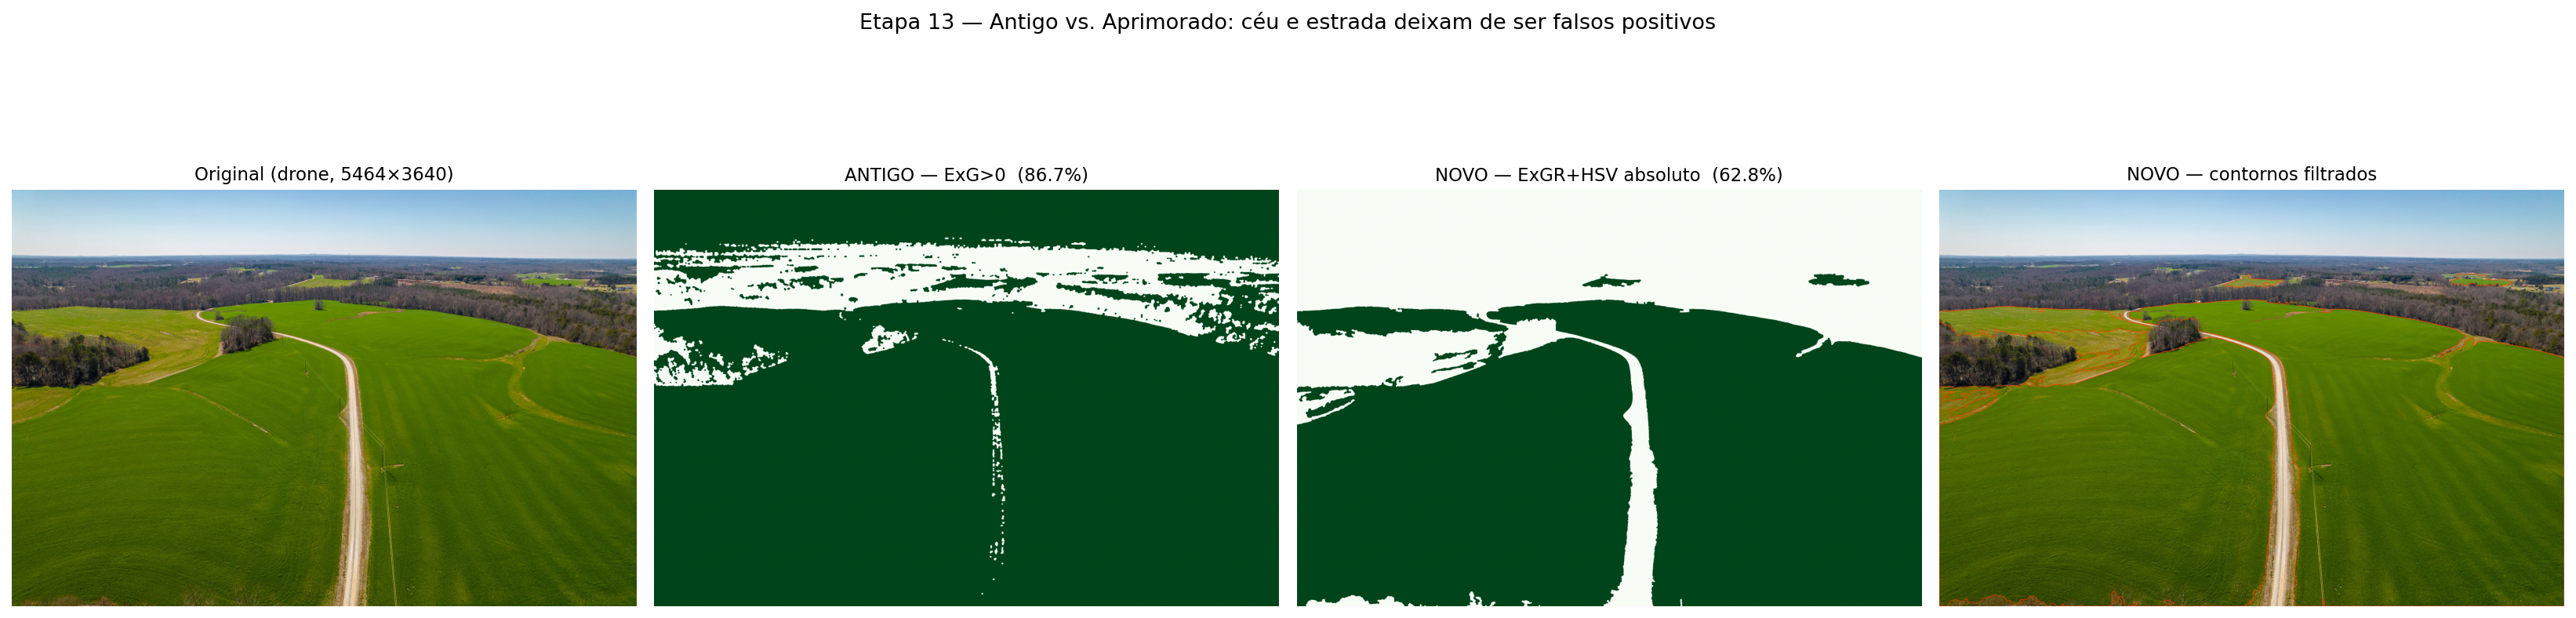
\includegraphics[width=\textwidth]{segmentacao_aprimorada.png}
\caption{Antigo \emph{vs.} aprimorado: o céu e a estrada deixam de ser classificados como
vegetação. Da esquerda para a direita: original, máscara ingênua, máscara final e contornos
filtrados sobre a imagem.}
\label{fig:aprimorada}
\end{figure}

\subsection{Análise multi-imagem}
O \emph{pipeline} foi aplicado às seis imagens do projeto (Tabela~\ref{tab:multi},
Figura~\ref{fig:multi}).

\begin{table}[H]
\centering
\caption{Análise multi-imagem com índice ExG (\emph{baseline}).}
\label{tab:multi}
\begin{tabular}{llcc}
\toprule
\textbf{Imagem} & \textbf{Origem} & \textbf{Veg.\ (\%)} & \textbf{VARI médio} \\
\midrule
WhatsApp 17:57       & celular & 8,86  & $-0{,}1365$ \\
WhatsApp 18:00       & celular & 97,08 & $-0{,}0016$ \\
paisagem-verde       & celular & 85,20 & $+0{,}2453$ \\
drone-campo-fazenda  & drone   & 87,85 & $+0{,}1397$ \\
drone-vegetação-densa& drone   & 99,35 & $+0{,}1744$ \\
drone-lavoura-solo   & drone   & 97,68 & $-0{,}0695$ \\
\bottomrule
\end{tabular}
\end{table}

\noindent
Destaca-se a divergência na imagem \texttt{drone-lavoura-solo}: o ExG indica 97,68\% de
vegetação, mas o VARI médio é negativo ($-0{,}0695$). Trata-se de uma superestimação do ExG
sobre solo avermelhado --- precisamente o falso positivo que a segmentação aprimorada corrige
(de 97,68\% para 39,1\%).

\begin{figure}[H]
\centering
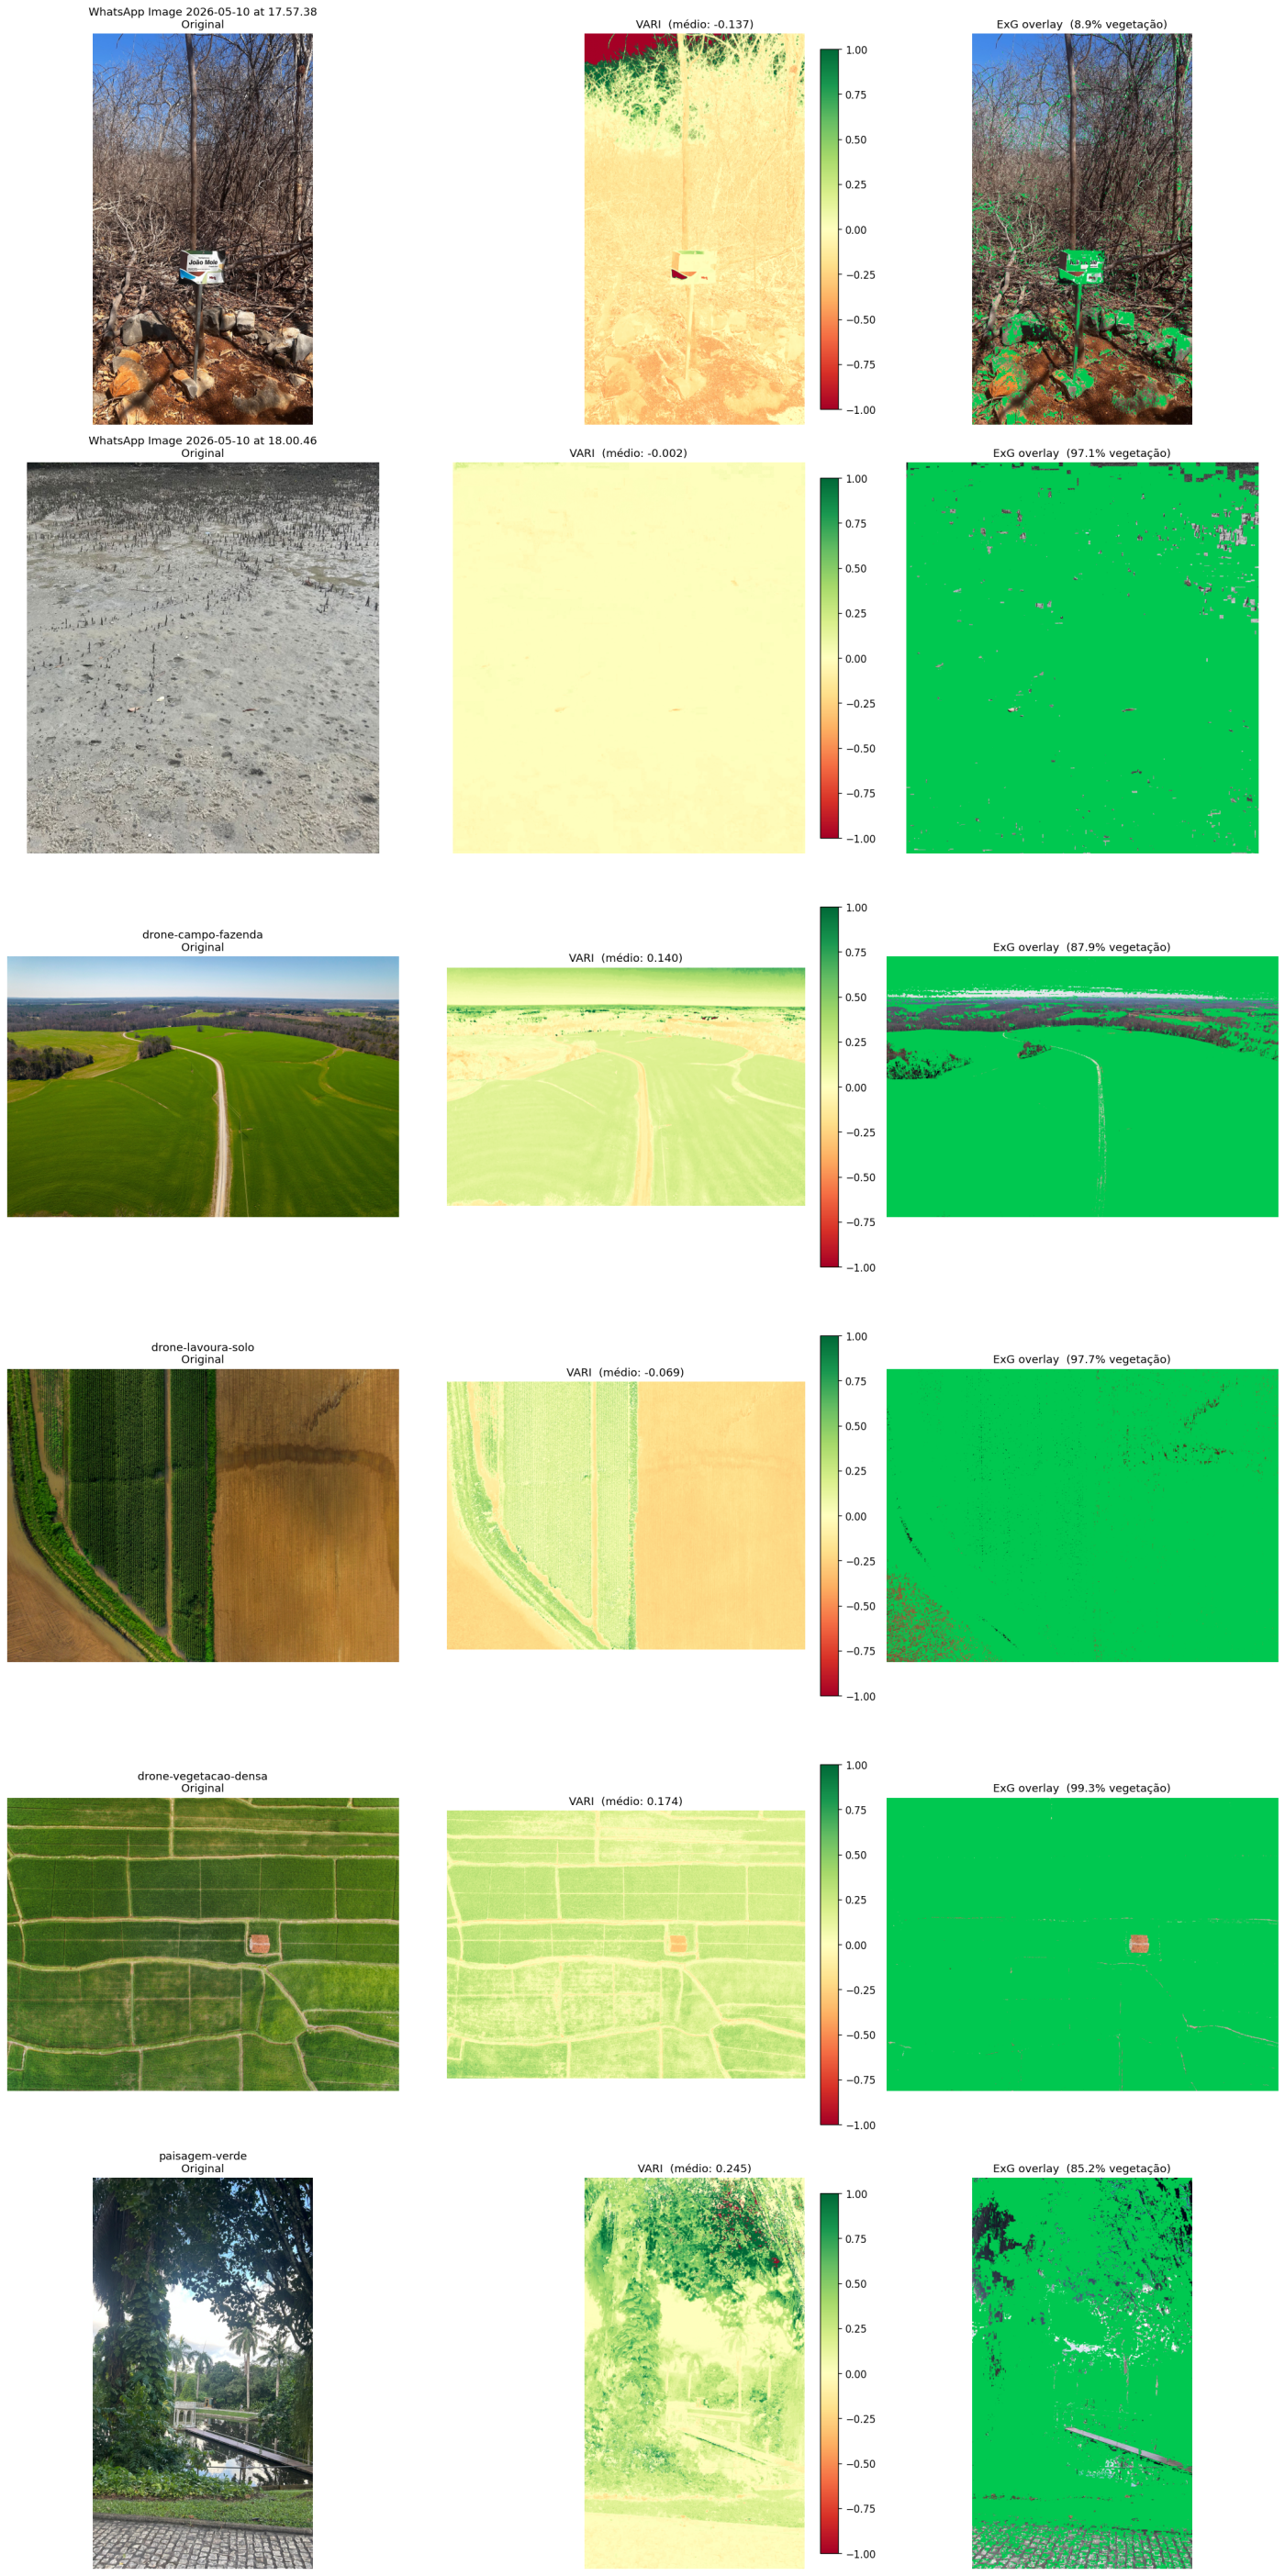
\includegraphics[width=0.85\textwidth]{analise_multi_imagem.png}
\caption{Original, VARI e ExG para as seis imagens (celular e drone).}
\label{fig:multi}
\end{figure}

\subsection{Pipeline completo}
A Figura~\ref{fig:grid} consolida todos os estágios em um único painel.

\begin{figure}[H]
\centering
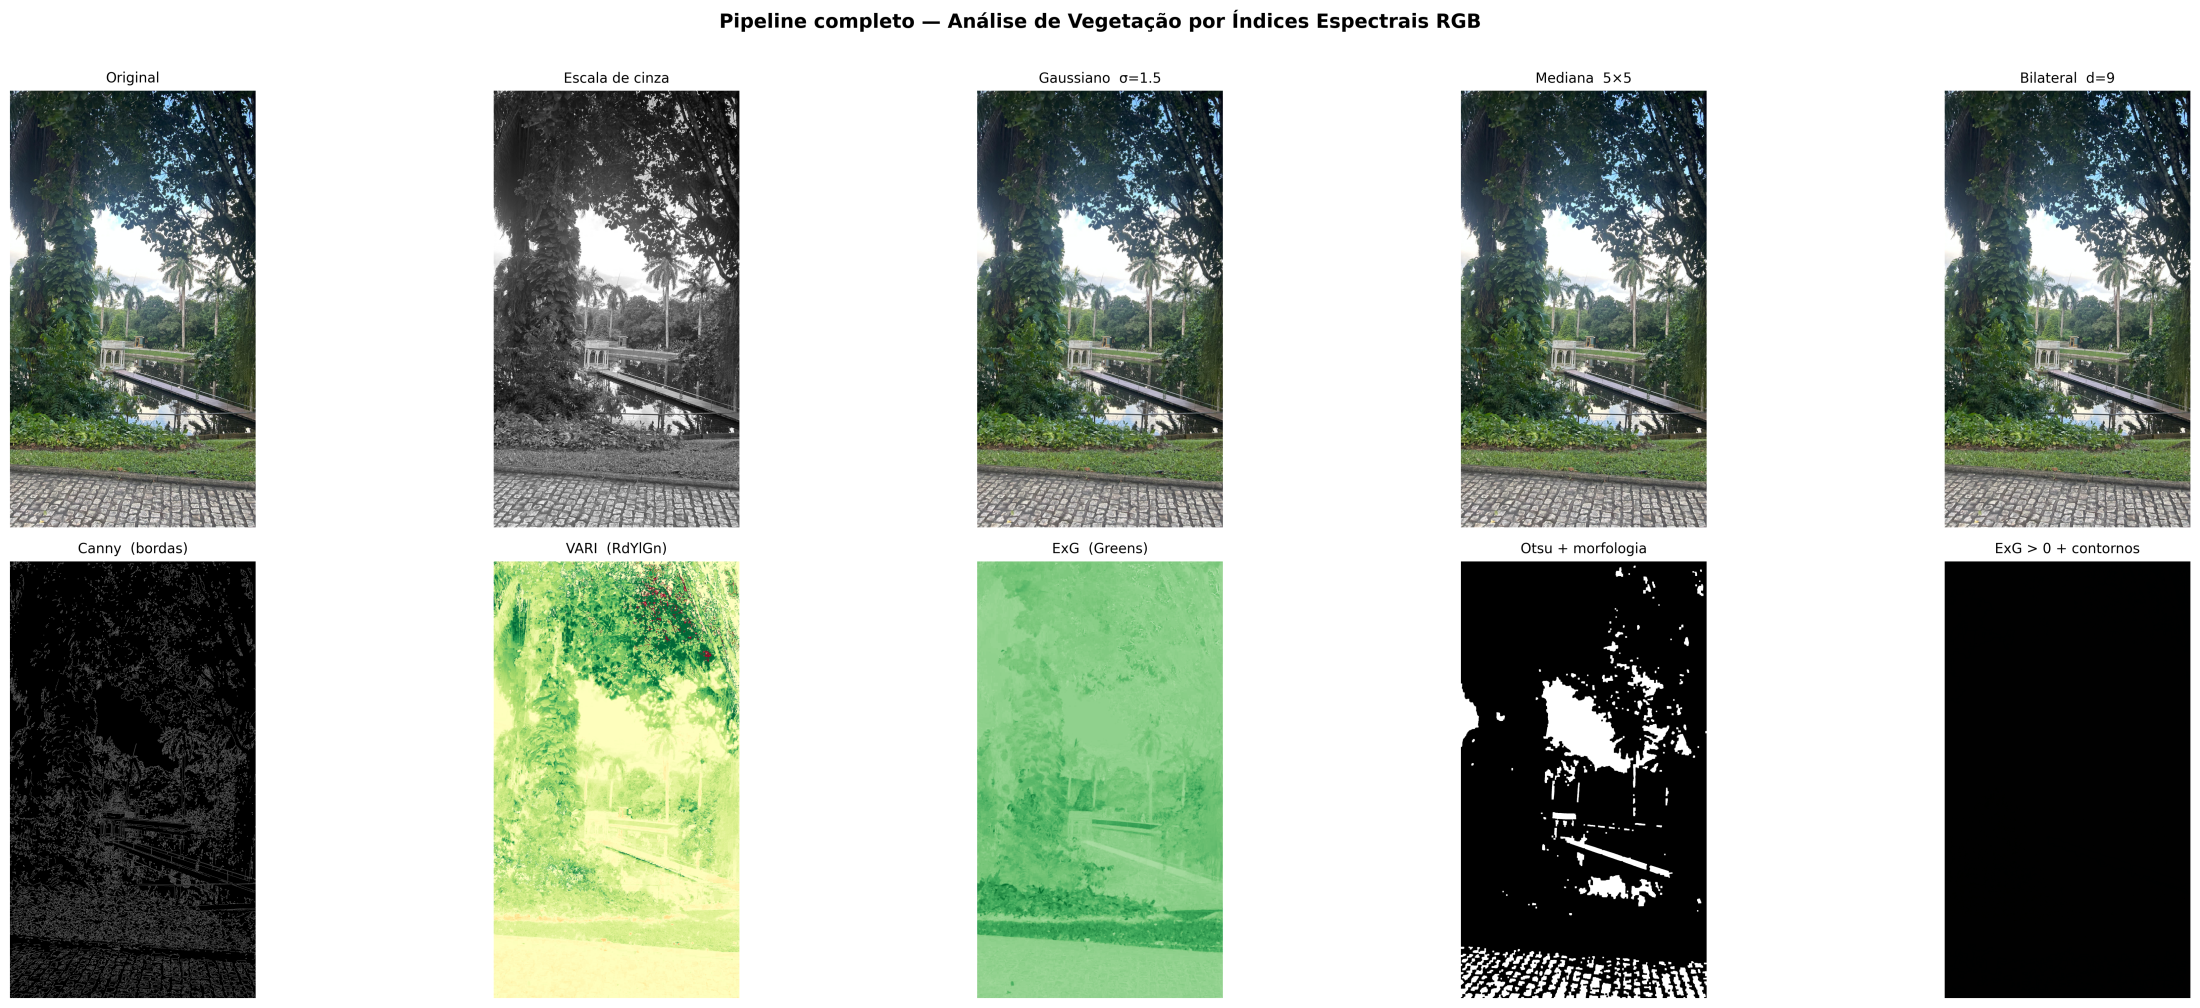
\includegraphics[width=\textwidth]{grid_pipeline_completo.png}
\caption{Grid comparativo $2\times5$ com todos os estágios do pipeline, gerado a 300 dpi.}
\label{fig:grid}
\end{figure}

% ════════════════════════════════════════════════════════════
\section{Análise Crítica}
% ════════════════════════════════════════════════════════════

Os experimentos sustentam três conclusões técnicas:

\begin{enumerate}
  \item \textbf{Crominância supera luminância.} Para vegetação em imagens RGB, índices de cor
        (ExG, VARI, ExGR) são superiores à limiarização de Otsu por brilho, que ignora a
        informação espectral que define a planta.
  \item \textbf{Testes absolutos superam testes relativos.} O limiar fixo erra por excesso
        (falsos positivos); o Otsu erra por falta em cenas uniformes (falsos negativos). A
        combinação \emph{absoluta} ExGR + HSV equilibra os dois extremos.
  \item \textbf{A imagem é parte do algoritmo.} Fotos de celular em ângulo oblíquo apresentam
        sombras e misturas de superfície que degradam os índices; imagens de drone em visada
        \emph{nadir} produzem resultados muito mais limpos, pois cada pixel representa uma única
        superfície.
\end{enumerate}

\paragraph{Limitações.} Imagens de satélite multiespectrais não são adequadas a estes índices,
projetados para câmeras RGB de superfície. O processamento interno de smartphones (HDR,
saturação) também pode distorcer a crominância.

% ════════════════════════════════════════════════════════════
\section{Conclusão}
% ════════════════════════════════════════════════════════════

O \emph{pipeline} desenvolvido cumpre todas as etapas propostas --- aquisição,
pré-processamento, análise de histograma, filtragem, detecção de bordas, segmentação e
visualização --- e vai além ao implementar índices espectrais especializados e uma segmentação
de alta precisão que elimina falsos positivos. Demonstrou-se que técnicas de processamento de
imagem extraem informação quantitativa de vegetação invisível a olho nu, e que a qualidade do
resultado depende tanto do algoritmo quanto da adequação da imagem de entrada. Como trabalho
futuro, sugere-se a validação com imagens de drone de alta resolução em diferentes culturas e
a integração com câmeras multiespectrais para o cálculo do NDVI.

% ════════════════════════════════════════════════════════════
\begin{thebibliography}{9}
% ════════════════════════════════════════════════════════════

\bibitem{gitelson2002}
GITELSON, A. A. \emph{et al.}
\textbf{Novel algorithms for remote estimation of vegetation fraction.}
Remote Sensing of Environment, v.~80, n.~1, p.~76--87, 2002.

\bibitem{woebbecke1995}
WOEBBECKE, D. M. \emph{et al.}
\textbf{Color indices for weed identification under various soil, residue, and lighting
conditions.}
Transactions of the ASAE, v.~38, n.~1, p.~259--269, 1995.

\bibitem{meyer2008}
MEYER, G. E.; NETO, J. C.
\textbf{Verification of color vegetation indices for automated crop imaging applications.}
Computers and Electronics in Agriculture, v.~63, n.~2, p.~282--293, 2008.

\bibitem{gonzalez2010}
GONZALEZ, R. C.; WOODS, R. E.
\textbf{Processamento Digital de Imagens.} 3.~ed. São Paulo: Pearson, 2010.

\bibitem{bradski2019}
BRADSKI, G.; KAEHLER, A.
\textbf{Learning OpenCV 4: Computer Vision with Python 3.} O'Reilly Media, 2019.

\bibitem{opencv}
OPENCV. \textbf{OpenCV Documentation.} Disponível em: \url{https://docs.opencv.org/4.x/}.

\bibitem{scikit}
SCIKIT-IMAGE. \textbf{Documentation.} Disponível em: \url{https://scikit-image.org/docs/stable/}.

\end{thebibliography}

\vspace{1cm}
\noindent\rule{\textwidth}{0.4pt}\\
\small \textbf{Repositório do projeto:}
\url{https://github.com/GilbertoPaiva/cv-vegetation-indices}

\end{document}
